\section{IMPLEMENTATION DETAILS}

\subsection{Dataset Explanation for MLP Classifier}

\subsubsection{Data Collection}
Web scraping emerged as a valuable tool in our data collection strategy, enabling us to
efficiently gather a diverse range of symptoms associated with various canine diseases
from reputable online sources. Leveraging Python libraries like Beautiful Soup and
Requests, we navigated through veterinary websites, academic articles, and reputable online platforms dedicated to pet care. This automated approach allowed us to accumulate a substantial volume of symptoms, providing a strong foundation for our dataset.

\subsubsection{Dataset Properties}
The dataset used for disease prediction in dogs is a structured collection of cases, where each case corresponds to a dog exhibiting a combination of symptoms. The dataset consists of rows and columns, with each row representing a unique case and each column representing a specific symptom. Those symptoms are associated with
diseases and verified by veterinarians. For each case, the presence or absence of each symptom is indicated by binary values: 1 for the presence of the symptom and 0 for the absence. Additionally, the target variable for each case is the disease that the dog is diagnosed with. Our database consists of three main tables as follows:

\begin{itemize}
\item Disease (ID, DiseaseCode, SymptomCode, Description)
\item Symptom (SymptomID, Description)
\item LearnedResult (ClusterID, InputNeuron, Strength)
\end{itemize}

\begin{table}[H] % Use [H] to place the table exactly here
\centering
\caption{Dataset Sample Table}
\label{tab:example}
\begin{tabular}{|p{0.8in}|p{1in}|p{1in}|p{1.2in}|}
    \hline
    ID & \textbf{symptoms\_id1} & \textbf{symptoms\_id2} & \textbf{symptoms\_id165} \\
    \hline
    Disease\_Id1 & 0 & 1 & 0 \\
    \hline
    Disease\_Id2 & 1 & 1 & 0 \\
    \hline
    Disease\_Id3 & 0 & 1 & 0 \\
    \hline
    . & 0 & 0 & 0 \\
    \hline
    . & 0 & 0 & 0 \\
    \hline
    Disease\_Id53 & 0 & 0 & 0 \\
    \hline
\end{tabular}

\end{table}


\subsubsection{Data Preprocessing for MLP Classifier}
Data preprocessing is a crucial step in preparing raw data for machine learning algorithms like the MLP (Multilayer Perceptron) Classifier in HelloPet. The primary goals include ensuring data quality, handling missing values, and normalizing or standardizing features to enable effective model training.
\subsubsection{Handling Missing Values}
In creating the dataset, symptoms related to each disease were gathered using web scraping. For each disease, symptoms that were relevant were kept, while those that didn't match were removed. This process aimed to make sure the dataset was complete and consistent, leaving no missing data to deal with later on.
\subsubsection{Normalization and Standardization}
The normalization and standardization processes are integral to ensuring that the input features are on a consistent scale. This is particularly important for algorithms like the MLP Classifier, which may be sensitive to varying magnitudes of features.

   \noindent\textbf{Normalization}\\
   The normalization process scales the input features to a range between 0 and 1. It is achieved using the formula:
   \begin{equation}
       X_{\text{norm}} = \frac{X - X_{\text{min}}}{X_{\text{max}} - X_{\text{min}}}
   \end{equation}
    where $X$ represents the original feature, $X_{\text{min}}$ and $X_{\text{max}}$ denote the minimum and maximum values of $X$, respectively.

    \noindent\textbf{Standardization}
    \begin{equation}
    X_{\text{std}} = \frac{X - \mu}{\sigma}     
    \end{equation}
    where $X$ represents the original feature, $\mu$ is its mean, and $\sigma$ is its standard deviation.

    \noindent Both normalization and standardization are applied to the input features to ensure consistent and comparable scales. So data preprocessing for the MLP Classifier in HelloPet involves handling missing values, normalizing, and standardizing input features. The normalization and standardization processes ensure that the MLP can effectively learn from the data, and the iterative training process refines the model for enhanced accuracy in recognizing subtle symptom combinations indicative of specific diseases.


\subsubsection{Data Splitting}
Data splitting is a crucial step in machine learning, including when working with an MLP classifier. It involves dividing your dataset into separate subsets for training and testing. The main goal is to assess the model's performance on unseen data and avoid overfitting. Our dataset is split as
% \vspace{-0.8em}
\begin{itemize}
    \item Training data: X\_train 4140 sample, 166 features
    \item Testing data:  X\_test 1035 samples, 166 features
    \item Training labels: y\_train shape 4140 labels
    \item Testing labels: y\_test 1035 labels
\end{itemize}
% \vspace{-1em}
\subsubsection{Model Training and Evaluation}
We initialized the MLP classifier with one hidden layer of 225 neurons. The model was trained using the training set for a maximum of 1000 iterations. The training process involved adjusting the weights and biases of the network to minimize the training loss and fit the data. The model was initialized with the following parameters:
% \vspace{-0.8em}
\begin{itemize}
    \item Hidden Layer Sizes: 225
    % \item Maximum Iterations: 1000
    \item Occurred Iterations: 200
    \item Random State: 42
\end{itemize}
% \vspace{-0.95em}
\subsubsection{Model Optimization}
Initially, the MLP classifier was trained on the default dataset, yielding around 40\% accuracy on testing data. In pursuit of enhancement, we systematically tuned hyperparameters, like increasing hidden layer sizes to 225 and maximum iterations to 1000. Additionally, L1 and L2 regularization with an alpha value of 1.5 were applied to the model to mitigate overfitting, enhancing model
performance through iterations and varied training-validation sets.

\subsection{Dataset Explanation of ResNet50}
\subsubsection{Data Collection}
The dataset utilized for the dog breed detection task was sourced from Kaggle, comprising a comprehensive collection of dog images covering 120 distinct breeds. Each breed in the dataset encompasses approximately 167 images, totaling a substantial corpus of 20,000 images. The images obtained from this dataset were obtained in their raw format and is required to be preprocessed to ensure suitability for subsequent processing steps.


\subsubsection{Model Setup}
The ResNet50 model is initialized with pre-trained weights from ImageNet, specified as weights = ResNet50\_Weights.IMAGENET1K\_V1. To understand the model's architecture, a summary is generated using torchinfo.summary. For input data, the model expects a tensor of size (1, 3, 256, 256), where the batch size is 1, there are 3 color channels, and the input image dimensions are 256x256. Certain layers within the model, including conv1, bn1, relu, maxpool, layer1, layer2, layer3, and layer4, are configured to not require gradients (requires\_grad = False). Furthermore, to adapt the model for dog breed classification, the last fully connected layer (model.fc) is replaced with a new sequential layer: nn.Linear(in\_features = 2048, out\_features = 120). This modification alters the output features to 120, aligning with the classification requirement for dog breeds.

\subsubsection{Model Modification} 
To facilitate model training for specific layers, the code loops through the selected layers, namely conv1, bn1, relu, maxpool, layer1, layer2, layer3, and layer4. Within this iteration, each layer's parameters undergo a setting adjustment where requires\_grad is set to False.
The iterative process systematically freezes these designated layers during the training phase. By setting requires\_grad = False, updates to the weights within these layers are withheld, ensuring that their learned features remain unchanged throughout the training process.
\vspace{1cm}
\begin{table}[ht]
    \centering
    \caption{Training Results}
    \label{tab:training_results}
    \begin{tabular}{|c|c|c|c|}
    \toprule
    \textbf{Epoch} & \textbf{Loss} & \textbf{Accuracy (\%)} \\
    \midrule
    1 & 1.8798 & 59.2 \\
    2 & 0.658 & 82.38 \\
    3 & 0.4924 & 85.6 \\
    4 & 0.4042 & 87.78 \\
    5 & 0.3479 & 89.43 \\
    6 & 0.2996 & 90.97 \\
    7 & 0.2638 & 91.79 \\
    8 & 0.2248 & 93.21 \\
    9 & 0.2444 & 93.15 \\
    10 & 0.2108 & 94.44 \\
    11 & 0.1704 & 94.48 \\
    12 & 0.1568 & 95.15 \\
    13 & 0.1494 & 95.3 \\
    14 & 0.1426 & 95.35 \\
    15 & 0.1399 & 95.47 \\
    \bottomrule
    \end{tabular}
    \end{table}
\newpage
\subsubsection{Training}
Firstly, the code defines the loss function utilized during training using nn.Cross Entropy Loss(). This loss function is well-suited for multi-class classification tasks, such as predicting the breed of dogs from a set of potential classes. Next, the code sets up the optimizer, employing the Adam optimization algorithm through torch.optim.Adam(). The optimizer fine-tunes the model's weights by iteratively adjusting them based on the computed loss and the specified learning rate (lr=0.001). Finally, the code specifies the number of training epochs, set to 15 in this instance (num\_epochs = 15). Throughout each epoch, the model undergoes multiple iterations or batches of training data, adjusting its parameters to improve its accuracy in predicting dog breeds.
\begin{figure}[H]
  \centering
  \begin{subfigure}{0.45\textwidth}
    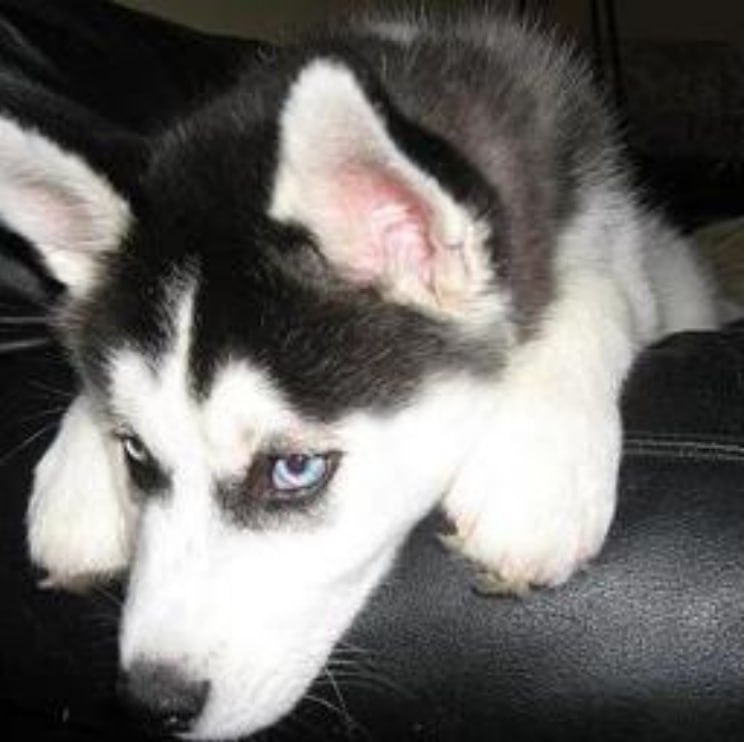
\includegraphics[width=0.9\linewidth]{img/training4.jpg}
    \caption{Original Image for Visualization}
  \end{subfigure}%
  \hfill
  \begin{subfigure}{0.45\textwidth}
    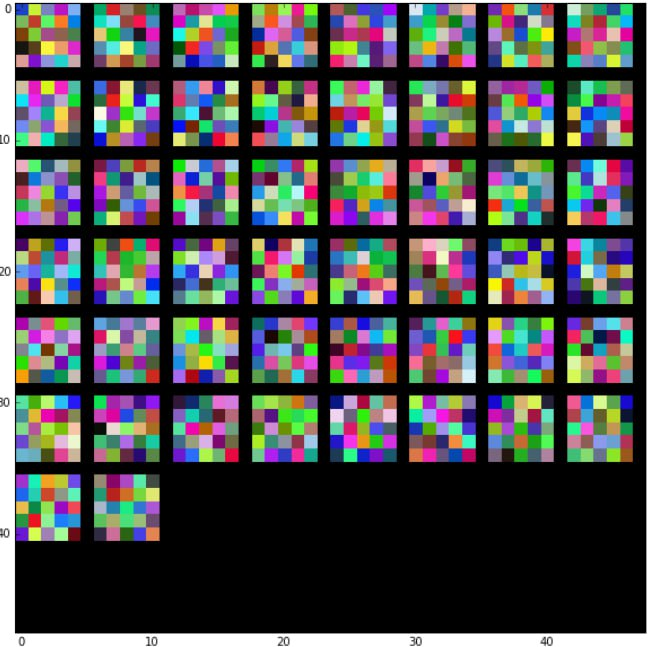
\includegraphics[width=.9\linewidth]{img/Training2.jpg}
    \caption{Visualizing First Layer}
  \end{subfigure}

  \label{fig:UI}
\end{figure}

\begin{figure}[ht]
  \centering
  \begin{subfigure}{0.45\textwidth}
    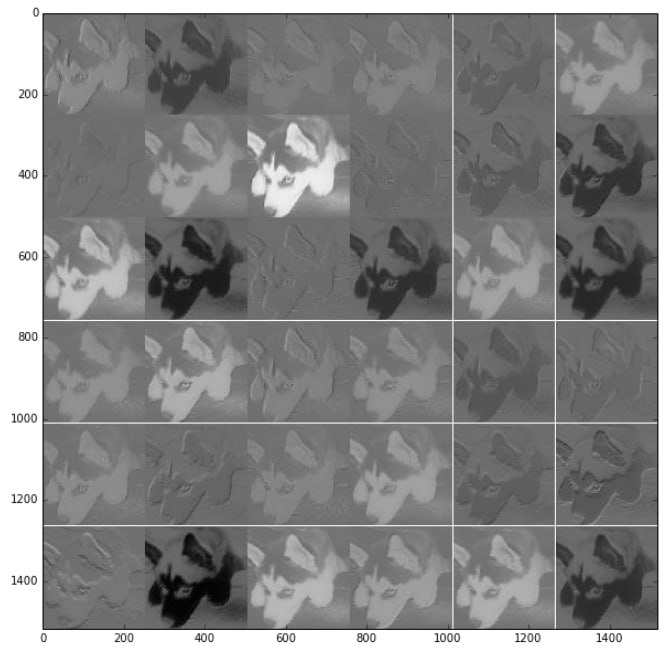
\includegraphics[width=.9\linewidth]{img/Traning3.jpg}
    \caption{Output from the First Layer}
  \end{subfigure}%
  \hfill
  \begin{subfigure}{0.45\textwidth}
    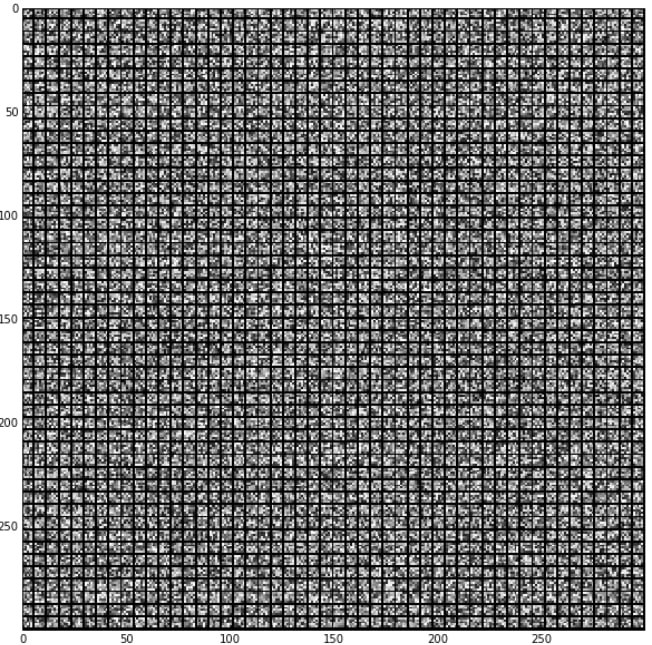
\includegraphics[width=.9\linewidth]{img/Training6.jpg}
    \caption{Final layer}
  \end{subfigure}
  \caption{Before and After Traning}
  \label{fig:UI}
\end{figure}
\newpage
\subsubsection{Experimental Results}
The training phase of the model for dog breed classification yielded promising outcomes across fifteen epochs. The progression of loss values showcased a consistent downward trend, starting at 1.8798 in the initial epoch and steadily decreasing to 0.1399 by the fifteenth epoch. Simultaneously, the accuracy of the model exhibited significant improvement, rising from 59.2\% to 95.47\% over the same period. This trend underscores the model's effective learning from the training dataset, marked by a reduction in prediction errors (lower loss) and an enhancement in its ability to accurately classify dog breeds (higher accuracy). 
\vspace{1cm}
\begin{figure}[H]
  \centering
  \begin{subfigure}{0.47\textwidth}
    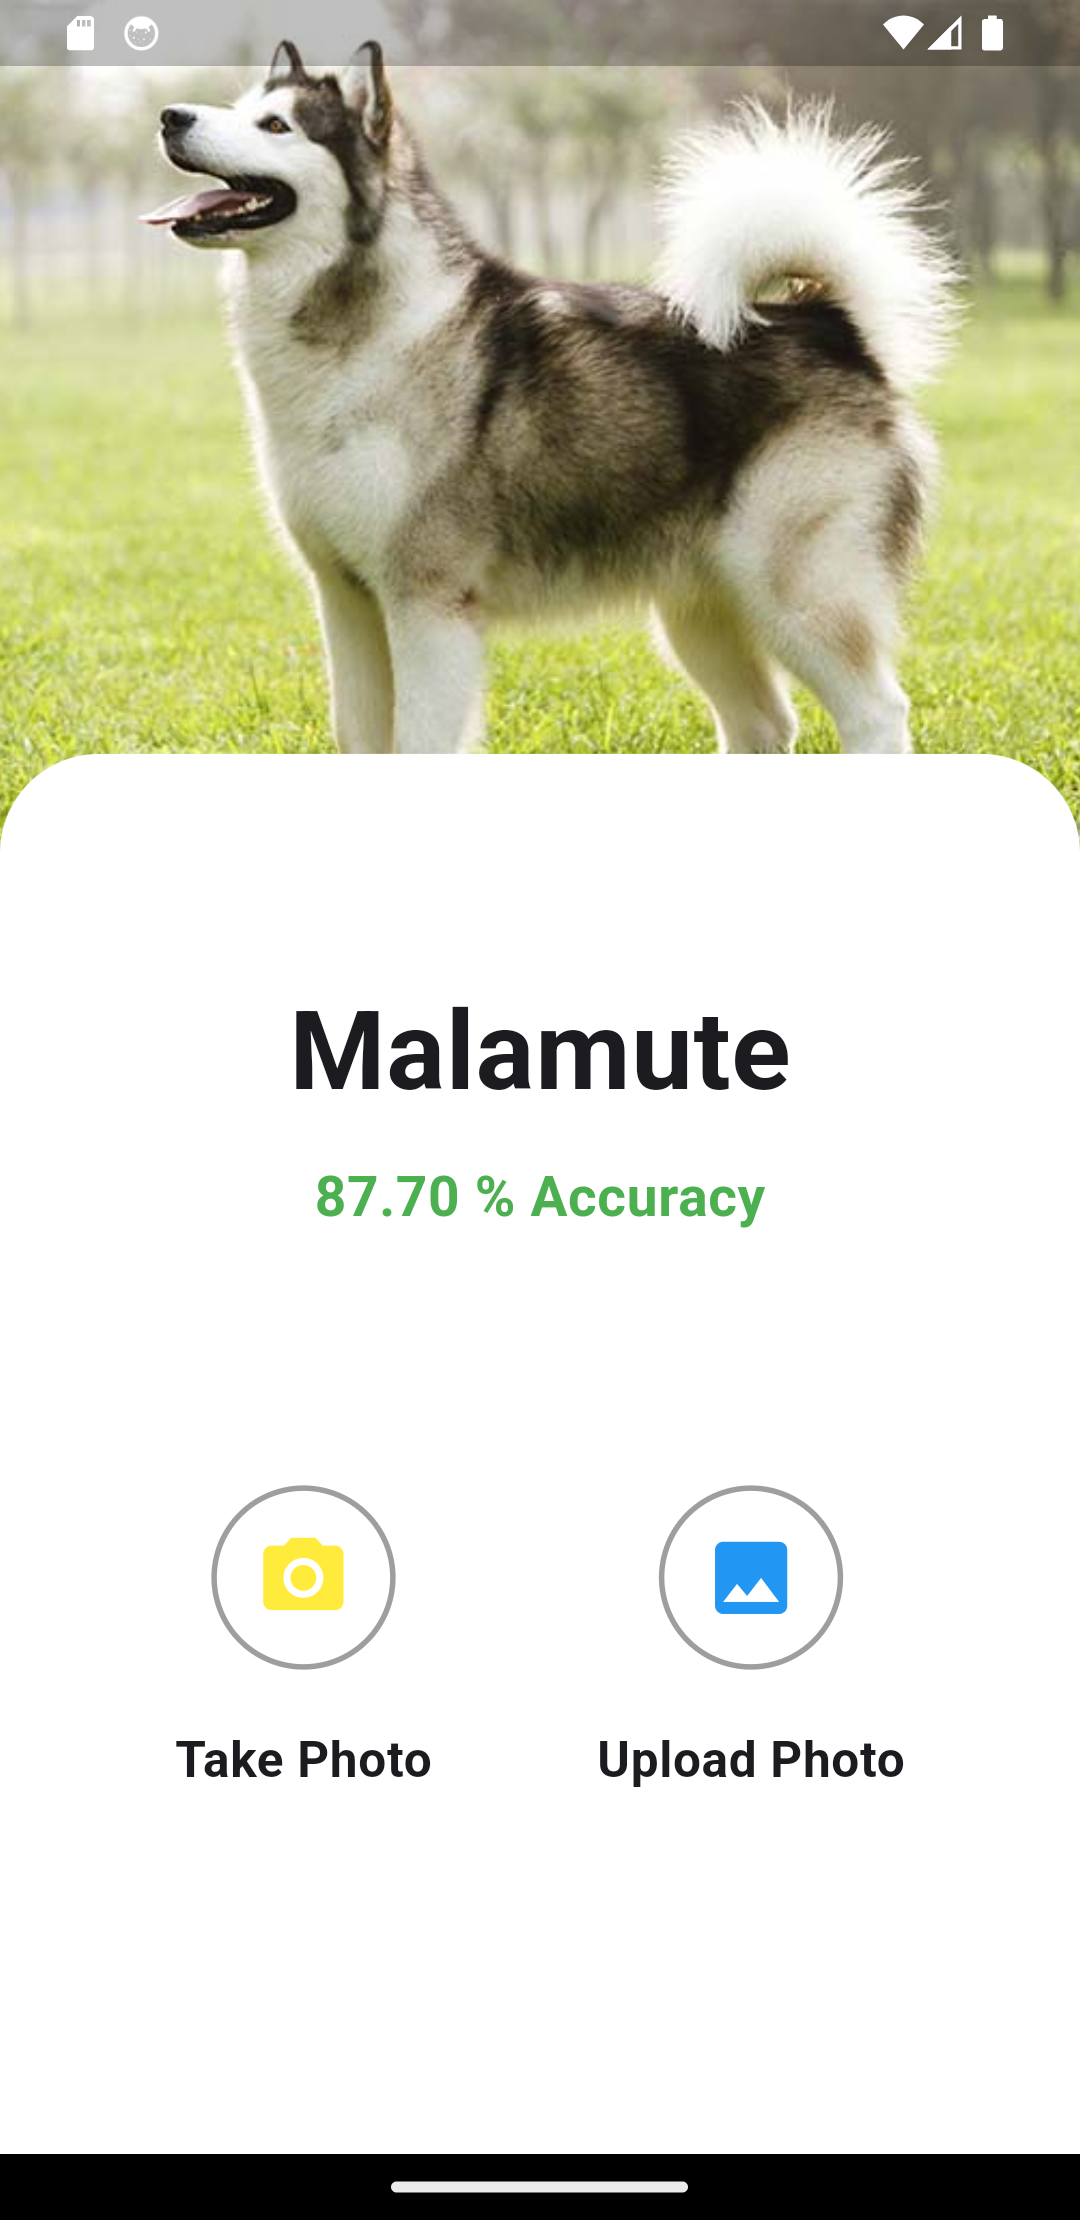
\includegraphics[width=\linewidth]{img/dog5.png}
    % \caption{Output from the First Layer}
  \end{subfigure}%
  \hfill
  \begin{subfigure}{0.47\textwidth}
    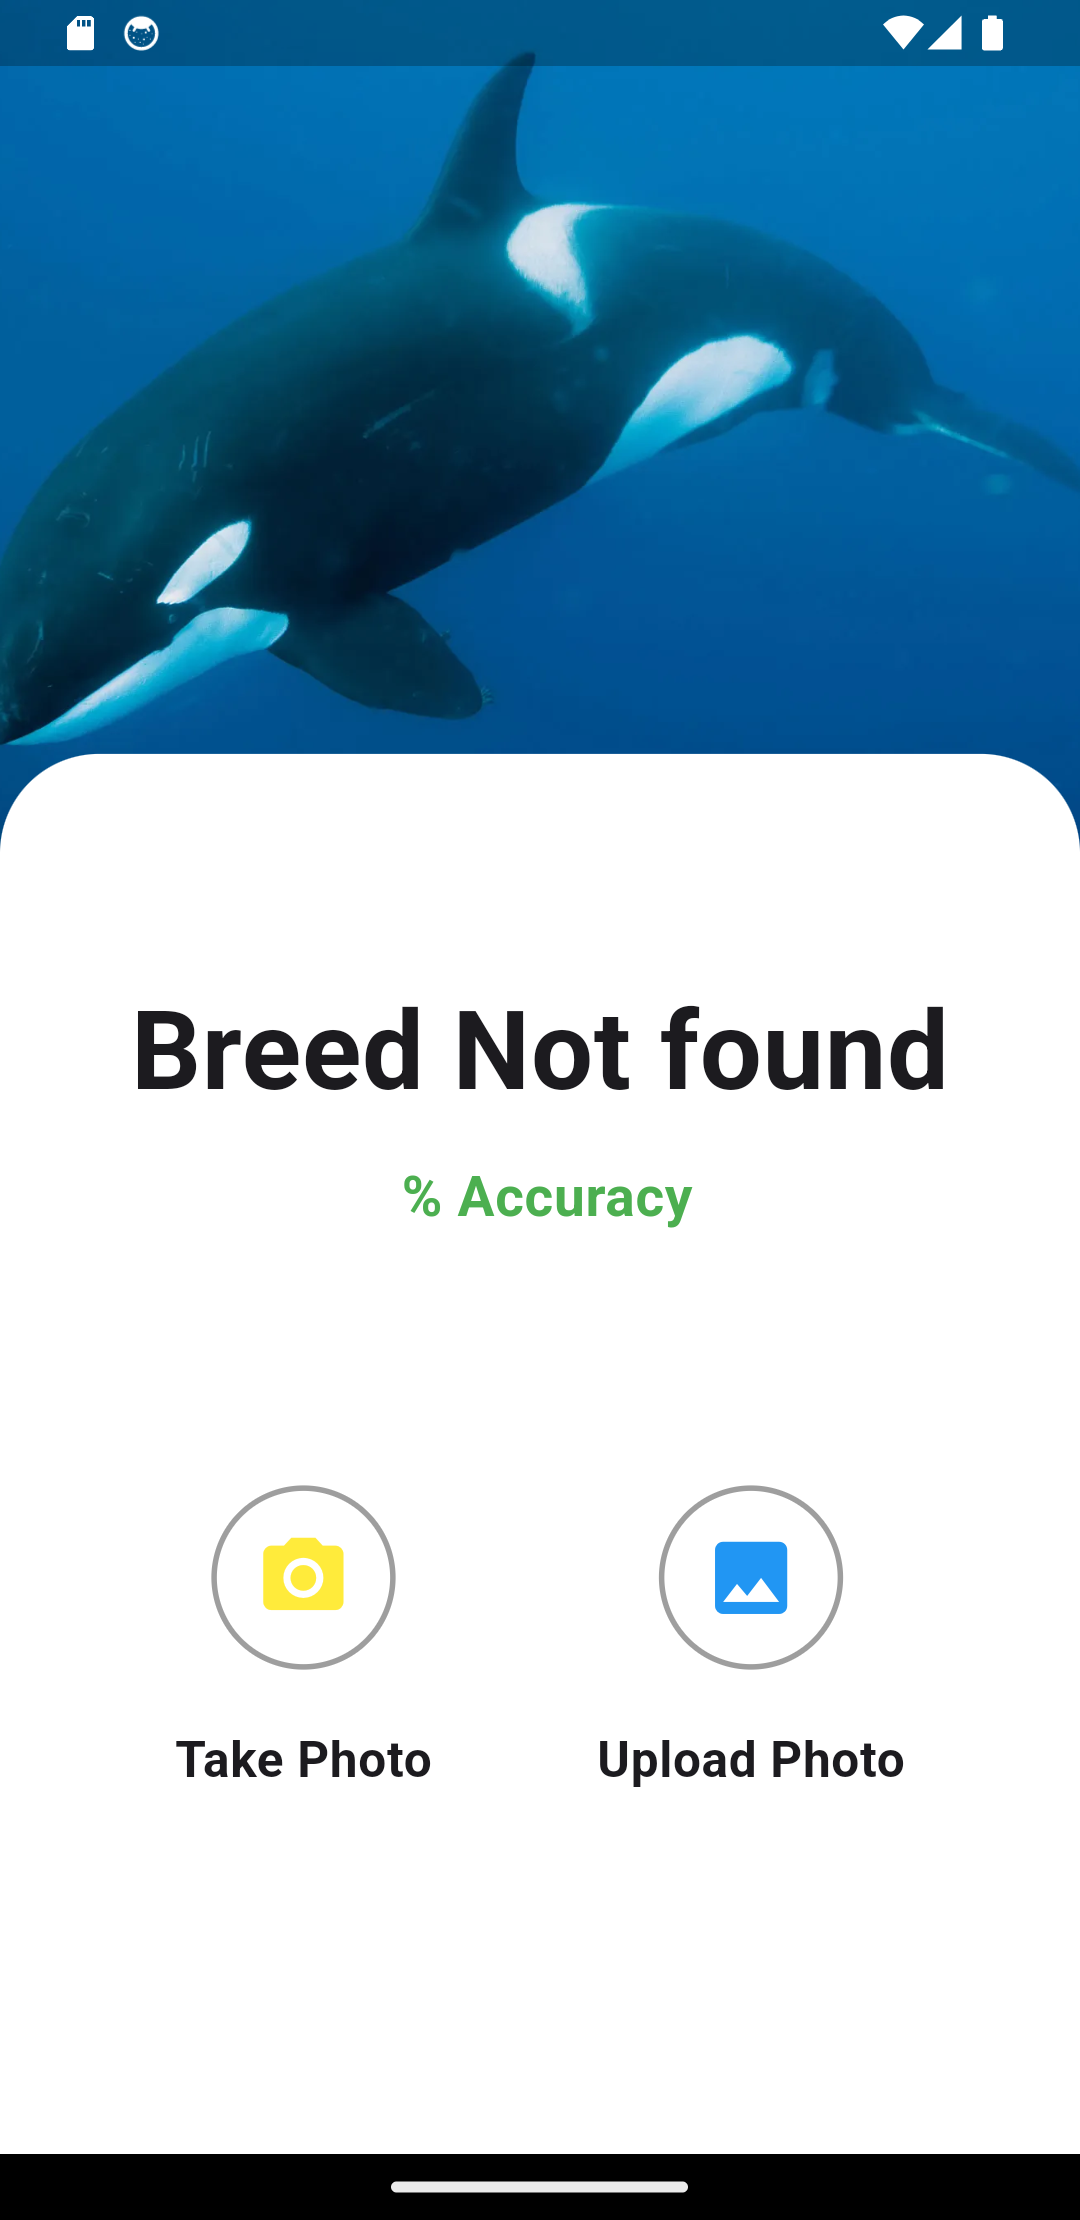
\includegraphics[width=\linewidth]{img/dog6.png}
    % \caption{Final layer}
  \end{subfigure}
  \caption{Breed Detection}
  \label{fig:UI}
\end{figure}

\newpage
\subsection{Dataset Explanation of Content based filtering}
\subsubsection{Data Collection}
The first step in building a recommendation system is to collect data. In this case, the data set is collected from web Scrap and also created manually.  This data will be used as the basis for the recommendation system.\\
\textbf{For example}, a database instance might contain the following information:

\noindent Post ID: 15\\
Community ID: 65 \\
Community Name: Hello-Pet\\
User ID: 25\\
User Name: PinkyAunty6\\
Title: Dog keeps vomitting in the morning\\
Content: After some advice. My dog keeps throwing up in the morning


\subsubsection{Data Prepossessing}
\textbf{Changing to Lower Case}\\
This step involves converting all text to lowercase. It is beneficial for ensuring uniformity and simplifying subsequent analysis, as it treats words regardless of their original case.

\noindent\textbf{Remove HTML Text Patterns using Regular Expressions (re)}\\
The objective is to eliminate HTML text patterns from the input. This process helps in cleaning the text data by removing any HTML tags or elements present, leaving only the essential text content.

\noindent\textbf{Remove Punctuation}\\
The removal of punctuation involves stripping away punctuation marks from the text. Punctuation is often irrelevant for certain analyses, and its removal helps focus on the actual content of the text.

\noindent\textbf{Handling Slang Words}\\
This step addresses the replacement of common slang abbreviations with their full forms. By doing so, it ensures that the text is represented in a more formal and standard manner, aiding in better understanding and analysis.

\noindent\textbf{Handling Emojis}\\
Handling emojis involves converting emojis to their text representations. This is done to ensure that emoji characters are transformed into a format that can be easily processed and understood, as required by certain text analysis tasks.

\noindent\textbf{Correct Spelling}\\
Correcting spelling mistakes is achieved using TextBlob. This process helps improve the overall quality of the text data by automatically correcting commonly occurring spelling errors, making the text more accurate and consistent.

\noindent\textbf{Stemming}\\
Stemming is the process of reducing words to their base or root form. In this case, Porter Stemming is applied to transform words, facilitating a simplified and more focused analysis by grouping related words together.

\noindent\textbf{Lemmatization}\\
Lemmatization involves reducing words to their base or dictionary form. The implementation uses WordNetLemmatizer to lemmatize words, ensuring that different inflections or variations of words are standardized for analysis.

\noindent\textbf{Tokenization and Removing Stop Words}\\
This step comprises two processes: tokenization and the removal of stop words. Tokenization breaks down the text into individual words, making it easier to analyze. Simultaneously, common English stop words are removed to exclude commonly used words that typically do not carry significant meaning in analysis.

\newpage
% \subsection{Sparse Matrix Creation}
\subsubsection{Sparse matrix creation}
The obtained values are then vectored into a sparse matrix. A sparse matrix is a matrix that contains mostly zeros, which is useful for processing large datasets efficiently. We can represent our data in the dataset as a sparse matrix, where each row corresponds to a post and each column corresponds to a unique user in the Community. The value in each cell represents the number of times the user appears in the corresponding product. Since most product will only contain a small subset of the users in our community, the matrix will be mostly zeros.
\vspace{1cm}
\begin{figure}[ht]
  \centering
  \includegraphics[width=0.7\textwidth]{img/method.pdf}
\centering
\includegraphics[width=0.7\textwidth]{img/matrix.pdf}
  \caption{matrix}
  \label{fig:matrix}
\end{figure}
\newpage
\subsubsection{Cosine similarity calculation}
For each vector in the sparse matrix, the similarity is calculated using the cosine similarity algorithm. Cosine similarity calculates the angle between each vector and returns a scalar value in the range of [-1, 1]. A higher value indicates greater similarity. Where value 1 represents itself. Cosine similarity is commonly used in text analysis and recommendation systems because it is invariant to the magnitude of the vectors, which means that it only considers the direction of the vectors. In the context of recommendation systems, the cosine similarity is calculated between the user vector and each of the item vectors in the sparse matrix. The resulting values represent the similarity between the user's preferences and each item in the dataset.
\vspace{1cm}
\begin{figure}[ht]
\centering
\includegraphics[width=0.7\textwidth]{img/distribution.pdf} 
\caption{Distribution Curve}
\label{fig:system-overview}
\end{figure}

\newpage
\subsection{Results Sorting}
The results for each vector are sorted, and the top 10 results are recommended, excluding the vector itself. This ensures that the recommended courses are not duplicates of the courses that the user has already taken. The items with the highest similarity scores are recommended to the user. The top N items, where N is usually set to 10, are recommended to the user, excluding any items that the user has already interacted with.

\vspace{1cm}
\begin{figure}[ht]
  \centering
  
  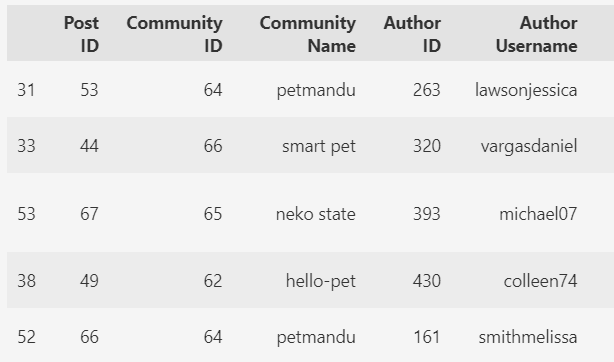
\includegraphics[width=0.9\textwidth]{img/1.png}
  \centering
  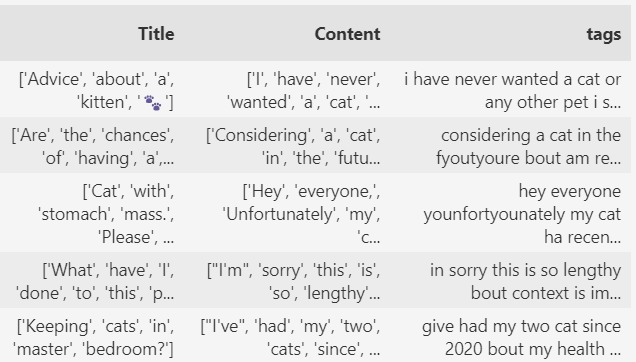
\includegraphics[width=0.9\textwidth]{img/2.png}
  \caption{Result Sorting}
  \label{fig:matrix}
\end{figure}